\documentclass[t]{beamer}
%\documentclass[finnish,english,handout]{beamer}

% Uncomment if want to show notes
% \setbeameroption{show notes}

\mode<presentation>
{
%  \usetheme{Copenhagen}
  % oder ...
  
  %\setbeamercovered{transparent}
  % oder auch nicht
}
\setbeamertemplate{itemize items}[circle]
\setbeamercolor{frametitle}{bg=white,fg=navyblue}



\usepackage[T1]{fontenc}
\usepackage[latin1]{inputenc}
\usepackage{times}
\usepackage{epic,epsfig}
\usepackage{subfigure,float}
\usepackage{amsmath,amsfonts,amssymb}
\usepackage{inputenc}
\usepackage{afterpage}
\usepackage{url}
\urlstyle{same}
\usepackage{amsbsy}
\usepackage{eucal}
\usepackage{rotating}
\usepackage{listings}
\usepackage{lstbayes}
\usepackage[all,poly,ps,color]{xy}
\usepackage{eurosym}
\usepackage{microtype}

% minted
\usepackage{minted}
\setminted{highlightcolor=yellow!25}
\newmintinline{r}{}
% The following is adjusted from
% https://tex.stackexchange.com/questions/548592/changing-all-colors-to-black-white-using-minted-sty
\makeatletter
\newcommand{\minted@style@bw}{%
  \renewcommand\fcolorbox[3][]{##3}%
  \renewcommand\textcolor[3][]{##3}%
  \color{gray}
}
% define new minted option "gray"
\minted@def@opt@switch{gray}
\fvset{formatcom*={%
  \ifthenelse{\equal{\minted@get@opt{gray}{true}}{true}}
  {\minted@style@bw}{}%
}}
\makeatother
% The following is ajusted from
% https://tex.stackexchange.com/questions/74459/remove-space-before-colorbox
\newcommand{\reducedstrut}{\vrule width 0pt height .9\ht\strutbox depth .9\dp\strutbox\relax}
\newcommand{\highlight}[1]{%
  \begingroup
  \setlength{\fboxsep}{0pt}%  
  \colorbox{yellow!30}{\reducedstrut\detokenize{#1}\/}%
  \endgroup
}

\usepackage{natbib}
\bibliographystyle{apalike}

\hypersetup{%
  bookmarksopen=true,
  bookmarksnumbered=true,
  pdftitle={Stan},
  pdfsubject={Bayesian data analysis},
  pdfauthor={Aki Vehtari},
  pdfkeywords={},
  pdfstartview={FitH -32768},
  colorlinks=true,
  linkcolor=navyblue,
  citecolor=navyblue,
  filecolor=navyblue,
  urlcolor=navyblue
}

% \definecolor{hutblue}{rgb}{0,0.2549,0.6784}
% \definecolor{midnightblue}{rgb}{0.0977,0.0977,0.4375}
% \definecolor{hutsilver}{rgb}{0.4863,0.4784,0.4784}
% \definecolor{lightgray}{rgb}{0.95,0.95,0.95}
% \definecolor{section}{rgb}{0,0.2549,0.6784}
% \definecolor{list1}{rgb}{0,0.2549,0.6784}
\definecolor{forestgreen}{rgb}{0.1333,0.5451,0.1333}
\definecolor{navyblue}{rgb}{0,0,0.5}
\renewcommand{\emph}[1]{\textcolor{navyblue}{#1}}

\graphicspath{{./figs/}}

\pdfinfo{            
  /Title      (Bayesian data analysis 4)
  /Author     (Aki Vehtari) % 
  /Keywords   (Bayesian probability theory, Bayesian inference, Bayesian data analysis)
}


\parindent=0pt
\parskip=8pt
\tolerance=9000
\abovedisplayshortskip=0pt

\setbeamertemplate{navigation symbols}{}
\setbeamertemplate{headline}[default]{}
\setbeamertemplate{headline}[text line]{\insertsection}
\setbeamertemplate{footline}[frame number]


\def\o{{\mathbf o}}
\def\t{{\mathbf \theta}}
\def\w{{\mathbf w}}
\def\x{{\mathbf x}}
\def\y{{\mathbf y}}
\def\z{{\mathbf z}}

\DeclareMathOperator{\E}{E}
\DeclareMathOperator{\Var}{Var}
\DeclareMathOperator{\var}{var}
\DeclareMathOperator{\Sd}{Sd}
\DeclareMathOperator{\sd}{sd}
\DeclareMathOperator{\Gammad}{Gamma}
\DeclareMathOperator{\Invgamma}{Inv-gamma}
\DeclareMathOperator{\Bin}{Bin}
\DeclareMathOperator{\Negbin}{Neg-bin}
\DeclareMathOperator{\Poisson}{Poisson}
\DeclareMathOperator{\Beta}{Beta}
\DeclareMathOperator{\logit}{logit}
\DeclareMathOperator{\N}{N}
\DeclareMathOperator{\U}{U}
\DeclareMathOperator{\BF}{BF}
\DeclareMathOperator{\Invchi2}{Inv-\chi^2}
\DeclareMathOperator{\NInvchi2}{N-Inv-\chi^2}
\DeclareMathOperator{\InvWishart}{Inv-Wishart}
\DeclareMathOperator{\tr}{tr}
% \DeclareMathOperator{\Pr}{Pr}
\def\euro{{\footnotesize \EUR\, }}
\DeclareMathOperator{\rep}{\mathrm{rep}}



\title[]{Bayesian data analysis}
\subtitle{}

\author{Aki Vehtari}

\institute[Aalto]{}

\begin{document} 

% \begin{frame}{rstanarm, brms, bambi, and formula syntax}

%   \vspace{-0.5\baselineskip}
%   \begin{itemize}
%   \item<+-> R (and systems before R) have used a formula syntax to describe
%     models, e.g.
%     \begin{itemize}
%     \item<+-> linear model: {\texttt{y $\sim$ 1 + x}\, or\, \texttt{y $\sim$ x}}
%     \item<+-> spline model: \texttt{y $\sim$ s(x)}
%     \item<+-> binomial model:\\ \texttt{deaths $\sim$ dosage, family = binomial}
%     \item<+-> hierarchical model:\\ \texttt{weight $\sim$ age + (age | ratid)}
%     \end{itemize}
%   \item<+-> \texttt{rstanarm} has pre-compiled Stan models
%     \begin{itemize}
%     \item no need to wait compilation time
%     \item limited size of the pre-compiled binaries in CRAN limits the number of model, family, prior combinations
%     \end{itemize}
%   \item<+-> \texttt{brms}
%     \begin{itemize}
%     \item extended formula syntax, e.g.\\
%     heteroscedastic linear model: {\texttt{bf(y $\sim$ x, sigma $\sim$ x)}}
%     \item user defined families
%     \item requires compilation of the generated Stan code
%     \end{itemize}
%   \item<+-> \texttt{bambi} implements formula syntax in Python
%   \end{itemize}

% \end{frame}

\begin{frame}{Rest of BDA3 and other reading}

  \begin{itemize}
  \item Rest of BDA3
  \item Gaussian process course in spring
    
  \item Regression and Other Stories
  \item Bayesian Workflow
  \end{itemize}

\end{frame}

\begin{frame}
  
  {\large\color{navyblue} Chapter 8: Modelling accounting for data collection}

  Highly recommended to read. Very informative, but also a dense chapter.
  
  \begin{itemize}
  \item We need to model the data collection unless it is ignorable
  \item We need to know when data collection is ignorable
  \item<2-> Data collection
    \begin{itemize}
    \item Sample surveys
    \item Designed experiments
    \item Randomization
    \item Observational studies
    \item Censoring and truncation
    \end{itemize}
  \end{itemize}
  
\end{frame}

\begin{frame}
  
  {\large\color{navyblue} Chapter 14: Introduction to regression models}

  \begin{itemize}
  \item Justification of conditional modeling
    \begin{itemize}
    \item if joint model factorizes $p(y,x|\theta,\phi)={\color{blue}p(y|x,\theta)}p(x|\phi)$\\
      we can model just ${\color{blue}p(y|x,\theta)}$
    \end{itemize}
  \item<2-> Gaussian linear model with conjugate prior
    \begin{itemize}
    \item the conditional posterior is multivariate normal
    \item with fixed prior on weights, the joint posterior is N-Inv-$\chi^2$
    \item<3-> these properties are sometimes useful and thus good to know,
      but with probabilistic programming less often needed
    \end{itemize}
  \item<4-> Bit on causal analysis (see much more in ROS Ch 18--21)
  \item<5-> Assembling matrix of explanatory variables (see also ROS Ch 10,12)
    \begin{itemize}
    \item identifiability, collinearity, nonlinear relations,
      indicator and categorical variables, interactions
    \item variable selection is not much discussed (extra lecture)
    \end{itemize}
  \item<6-> Regularization (see also ROS Ch 12)
    \begin{itemize}
    \item not much discussed (see extra lectures)
    \end{itemize}
  \item<7-> Unequal variances and correlations
  \end{itemize}
  
\end{frame}

\begin{frame}
  
  {\large\color{navyblue} Lasso and Bayesian lasso}

  \begin{itemize}
  \item Lasso is penalized maximum likelihood linear regression, with
    L1 one penalty where the amount penalty is adapted
    \begin{itemize}
    \item<2-> penalized maximum likelihood finds the mode given the
      penalty parameter, and is almost the same as maximum a
      posteriori
    \item<3-> when the amount of penalty is increased, marginal modes of
      weak effects go to zero first
    \item<4-> when the amount of penalty is increased, also the relevant
      coefficients are shrunk towards zero
    \item<5-> sometimes relaxed lasso is used, where after variable
      selection coefficients are re-estimated
    \end{itemize}
  \item<6-> Bayesian lasso uses Laplace distribution as prior
    \begin{itemize}
    \item Laplace prior is equivalent to L1 penalty
    \item<7-> but the Bayesian inference includes distribution for
      parameters and that distribution doesn't shrink to a point at
      zero, even if the mode would be at zero
    \item<8-> empirically better results obtained with more
      sparse priors
    \item<9-> it's best to separate selection of sensible prior, good
      posterior inference, and the decision analysis of which
      variables are important
    \end{itemize}
  \end{itemize}
  
\end{frame}

\frame{

  {\Large\color{navyblue} Sparse priors}

  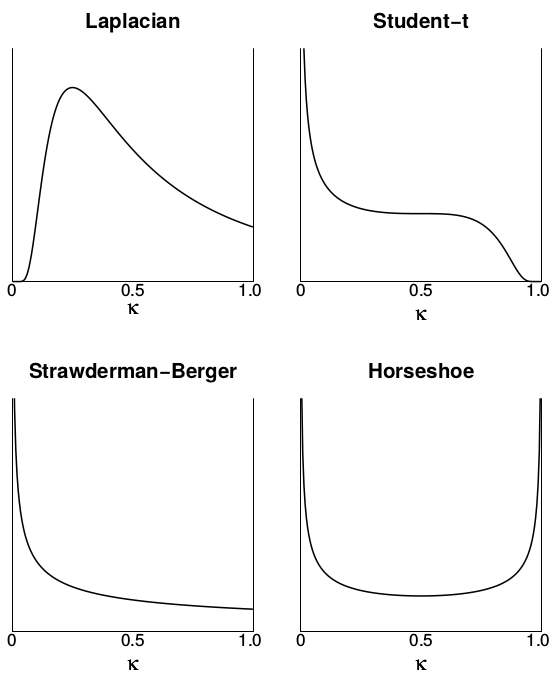
\includegraphics[width=6cm]{kappas.png}\\
  from Carvalho, Polson, Scott (2009).

}
\frame{

  {\Large\color{navyblue} Regularized horseshoe}

  \vspace{-0.5\baselineskip}
  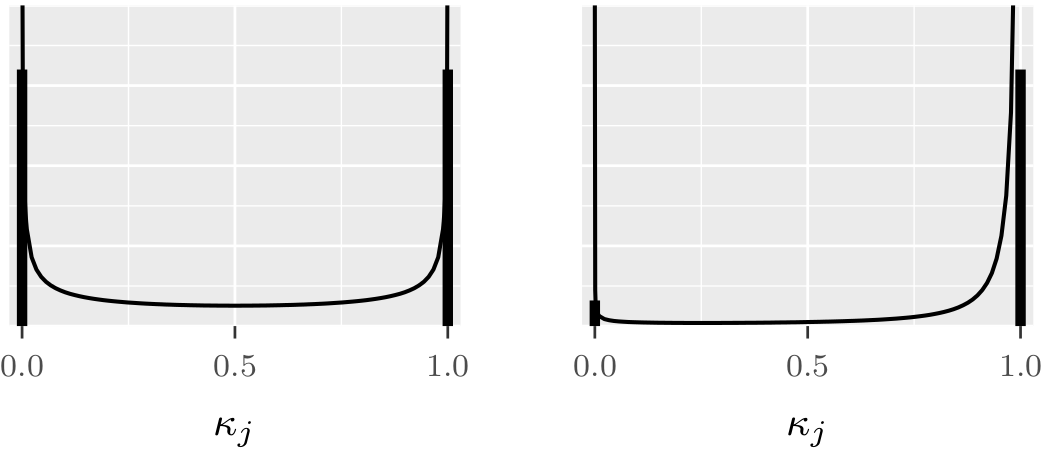
\includegraphics[width=6.5cm]{hs_vs_spikeandslab.png}\\
  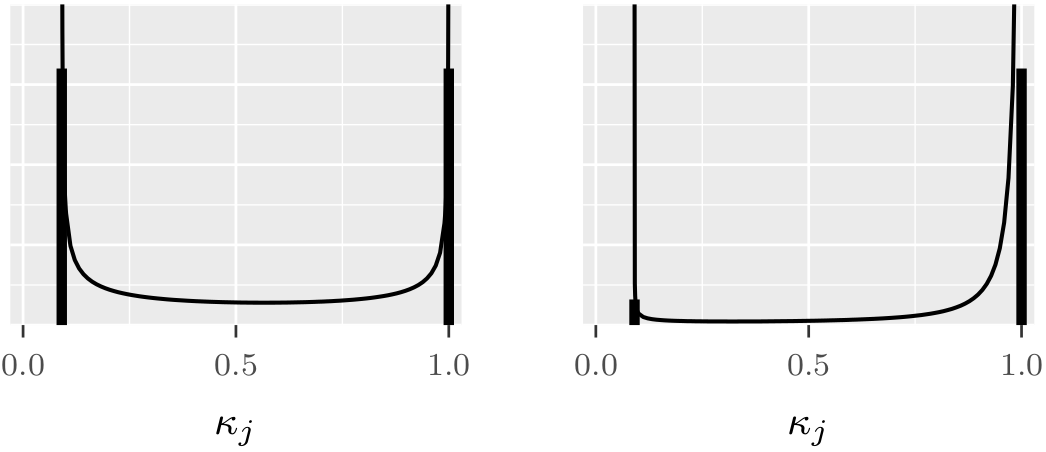
\includegraphics[width=6.5cm]{rhs_vs_spikeandslab.png}

  \vspace{-0.5\baselineskip}
  \begin{itemize}
  \item 
  {\small Piironen and Vehtari (2017). Sparsity information and
      regularization in the horseshoe and other shrinkage priors. In
      Electronic Journal of Statistics, 11(2):5018-5051. \href{https://projecteuclid.org/euclid.ejs/1513306866}{Online}}
  \item {\small\texttt{rstanarm}: \texttt{prior=hs()}}
  \item {\small\texttt{brms}: \texttt{prior=horseshoe()}}
  \end{itemize}
  

}

\frame{

  {\Large\color{navyblue} Projpred selection vs. Lasso}

  See projpred in an extra lecture
  
Simulated regression data \\�
$n=50$, $p=500$, $p_\text{rel} = 150$, $\rho=0.5$

\vspace{0.5em}

  \makebox[12.1cm][t]{
    \hspace{-0.5cm}
  \begin{minipage}{0.99\textwidth}
      \only<1>{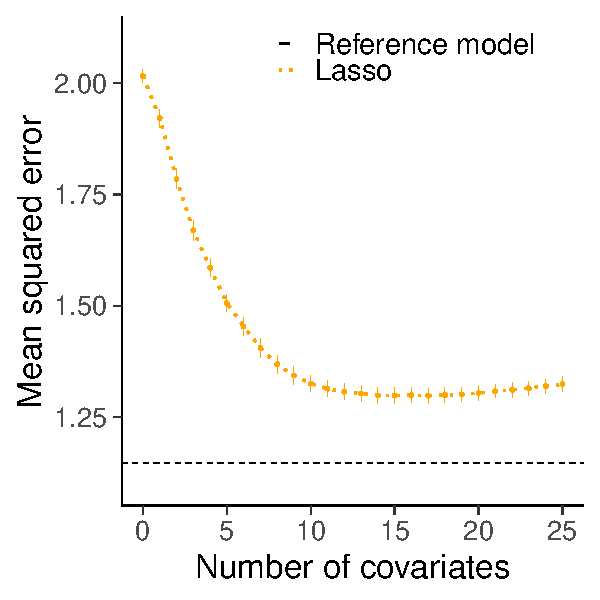
\includegraphics[width=5.5cm]{vslasso1rmse.pdf}}
      \only<2>{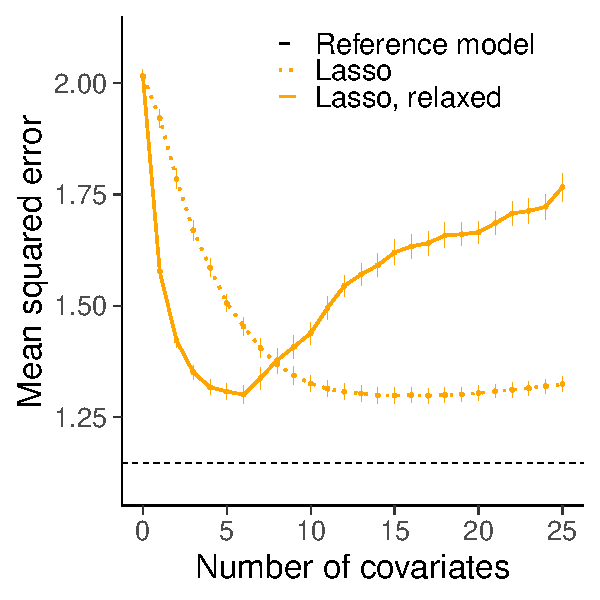
\includegraphics[width=5.5cm]{vslasso2rmse.pdf}}
      \only<3->{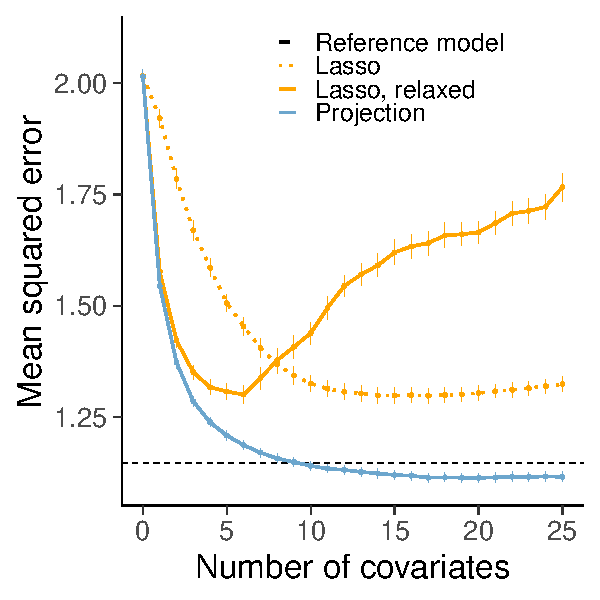
\includegraphics[width=5.5cm]{vslasso3rmse.pdf}}
      \uncover<4>{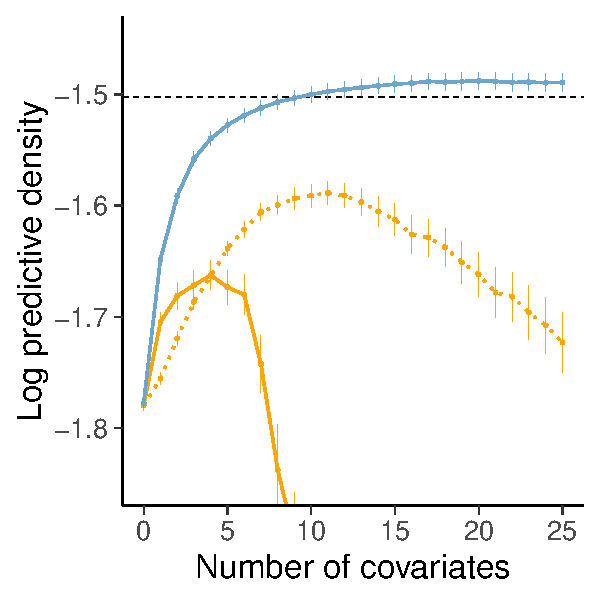
\includegraphics[width=5.5cm]{vslasso3mlpd.pdf}}
  \end{minipage}
  }
  
}

\begin{frame}
  
  {\large\color{navyblue} Chapter 15: Hierarchical linear models}

  \begin{itemize}
  \item Since you know hierarchical models, theory is easy
  \item With probabilistic programming computation is also easy
    \begin{itemize}
    \item BDA3 discusses some other computational issues
    \item section on transformations for HMC is relevant\\ (see also
      Stan user guide 21.7 Reparameterization)
    \end{itemize}
  \item<2-> Fixed, random, and mixed effects models
    \begin{itemize}
    \item we don't recommend using these terms, but they are so
      popular that it's useful to know them
    \end{itemize}
    \uncover<3->{\hspace{-1cm}\small
        \begin{tabular}[t]{ll}
     \rinline/y ~ 1 + x/ & fixed / population effect; pooled model\\
     \rinline/y ~ 1 + (0 + x | g)/ & random / group effects \\
     \rinline/y ~ 1 + x + (1 + x | g)/ & mixed effects; hierarchical model 
        \end{tabular}
      }
      \vspace{1\baselineskip}
  \item<3-> ANOVA in section 15.6 (see also {\tt stan\_aov})
  \end{itemize}
  
\end{frame}

\begin{frame}
  
  {\large\color{navyblue} Chapter 16: Generalized linear models}

  \begin{itemize}
  \item Bioassay model is an example of GLM
  \item<2-> Components: (see also ROS Ch 13--15)
    \begin{itemize}
    \item[1.] The linear predictor $\eta = X\beta$
    \item<3->[2.] The link function $g(\cdot)$ and $\mu = g^{-1}(\eta)$
    \item<4->[3.] Outcome distribution model with location parameter $\mu$
      \begin{itemize}
      \item<5-> the distribution can also depend on dispersion
        parameter $\phi$
      \item<6-> originally just exponential family distributions
        (e.g. Poisson, binomial, negative-binomial), which all have
        natural location-dispersion parameterization
      \item<7-> after MCMC made computation easy, GLM can refer to
        models where outcome distribution is not part of exponential
        family and dispersion parameter may have its own latent linear
        predictor
      \end{itemize}
      \uncover<8->{\hspace{-1cm}\small
     \rinline/deaths ~ dosage, family = binomial/ \\
        }
      \item<9-> Hierarchical GLM natural extension
    \item<10-> 16.3 Weakly informative priors section is excellent
      although the recommendation on using Cauchy has changed (see
      \url{https://github.com/stan-dev/stan/wiki/Prior-Choice-Recommendations})
      
    \end{itemize}
  \end{itemize}

  
\end{frame}

\begin{frame}
  
  {\large\color{navyblue} Chapter 17: Models for robust inference}

  \begin{itemize}
  \item For example (see also ROS Ch 15)\\
    \begin{tabular}[t]{lcl}\small
      normal & $\rightarrow$ & $t$-distribution\\
      Poisson & $\rightarrow$ & negative-binomial \\
      binomial & $\rightarrow$ & beta-binomial \\
      probit & $\rightarrow$ & logistic / robit 
    \end{tabular}
  \item<2-> Computation with MCMC easy
    \begin{itemize}
    \item posterior can be multimodal
    \item<3-> rstanarm doesn't have $t$-distribution for outcome, but brms
      has
    \end{itemize}
  \end{itemize}

  
\end{frame}

\begin{frame}
  
  {\large\color{navyblue} Chapter 18: Models for missing data}

  \begin{itemize}
  \item Extends the data collection modelling from Chapter 8
  \item Useful terms 
    \begin{itemize}
    \item<2-> Missing completely at random (MCAR)\\
      missingness does not depend on missing values or other observed
      values (including covariates)
    \item<3-> Missing at random (MAR)\\
      missingness does not depend on missing values but may depend on
      other observed values (including covariates)
    \item<4-> Missing not at random (MNAR)\\
      missingness depends on missing values
    \end{itemize}
  \item<5-> Multiple imputation
    \begin{itemize}
    \item[1.] make a model predicting missing data
    \item[2.] sample repeatedly from the missing data model to generate
      multiple imputed data sets
    \item[3.] make usual inference for each imputed data set
    \item[4.] combine results
    \item<6-> \texttt{mice} package is ver flexible
    \end{itemize}
  \item<7-> \texttt{brms} can handle some missing data
  \end{itemize}
  
\end{frame}

\begin{frame}
  
  {\large\color{navyblue} Chapter 21: Gaussian process models}

  \begin{itemize}
  \item Gaussian process is 
    \begin{itemize}
    \item infinite dimensional extension of normal distribution
    \item useful prior for non-linear functions
    \item for any finite number of variables, the marginal is
      multivariate normal
    $f_1,\ldots,f_n  \sim \N\left(\mu( x_1,\ldots, x_n), K(x_1,\ldots,x_n) \right)$
    \end{itemize}
  \item<2-> Often a priori $\mu = 0$
  \item<3-> Prior for smooth non-linear functions, e.g. with\\
      $k(x,x') = \tau^2 \exp\left(-\,\frac{| x - x' |^2}{2l^2}\right)$
  \end{itemize}
  \vspace{-1\baselineskip}
 \only<4>{\hspace{-0.5cm}\includegraphics[width=12cm]{gpprior-eps-converted-to.pdf}}
 \only<5>{\hspace{-0.5cm}\includegraphics[width=12cm]{gpposterior-eps-converted-to.pdf}}
  
\end{frame}

\begin{frame}
  
  {\large\color{navyblue} Chapter 21: Gaussian process models}

  \begin{itemize}
  \item Conditional on covariance function parameter the posterior is
    just multivariate normal
    \begin{itemize}
    \item need to make inference for covariance function parameters
      given the marginal likelihood
    \item the exact computation of the marginal likelihood scales
      $O(N^3)$
    \end{itemize}
  \end{itemize}
  
\end{frame}


\begin{frame}

  \vspace{-0.75\baselineskip}
  \begin{itemize}
  \small
  \item Easy to make additive models\\
    $y_t(t) = f_1(t) + f_2(t) + f_3(t) + f_4(t) + f_5(t) +\epsilon_t$\\
    \includegraphics[width=7.5cm]{birthsnewbw-eps-converted-to.pdf}
  \end{itemize}  

\end{frame}

\begin{frame}
  
  {\large\color{navyblue} Chapter 21: Gaussian process models}

  \begin{itemize}
  \item For non-Gaussian outcome models similar extension as GLMs
  \item Survival model example:
  \end{itemize}

  \includegraphics[width=8cm]{gp_leukemia-eps-converted-to.pdf}
  
\end{frame}

\begin{frame}
  
  {\large\color{navyblue} GPs in Stan}

  \begin{itemize}
  \item GP specific software (e.g. GPy, GPflow, GPyTorch) scale
    computationally better for GPs than Stan
  \item Stan has some built-in covariance functions
  \item Hilbert space basis function approximation of GPs is fast for 1D-3D (\href{https://arxiv.org/abs/2004.11408v2}{Riutort-Mayol et al., 2022})
    \begin{itemize}
    \item \href{https://avehtari.github.io/casestudies/Birthdays/birthdays.html}{Birthday example}
    \item \href{https://avehtari.github.io/casestudies/Motorcycle/motorcycle_gpcourse.html}{Motorcycle example}
    \end{itemize}
  \item In case of non-Gaussian outcome models, sampling of latent
    variables can be slow (Laplace integration over the latents coming)
  \item<2-> \texttt{brms}:
    \begin{itemize}
    \item covariance matrix based computation:\\ \rinline/y ~ gp(x)/
    \item Hilbert space basis function approximation:\\
    \rinline/y ~ gp(x, k=20)/ 
    \end{itemize}
  \end{itemize}
  
\end{frame}

\begin{frame}{Regression and Other Stories}

  \begin{itemize}
  \item Gelman, Hill, and Vehtari (2020). Regression and Other Stories.
    \begin{itemize}
    \item uses Bayesian inference, but maths and computation is minimal
    \item focuses on different models and how think about modeling
    \item a lot of different examples
    \item \url{https://avehtari.github.io/ROS-Examples/}
    \end{itemize}
  \end{itemize}
  
\end{frame}

\begin{frame}{Bayesian workflow}

  \vspace{-\baselineskip}\footnotesize
  Gelman, Vehtari, Simpson, Margossian, Carpenter, Yao, Kennedy,
  Gabry, B�rkner, and Modr�k (2020). Bayesian
  workflow. \href{https://arxiv.org/abs/2011.01808}{arXiv:2011.01808}
  
  \centering
  \vspace{-0.5\baselineskip}
  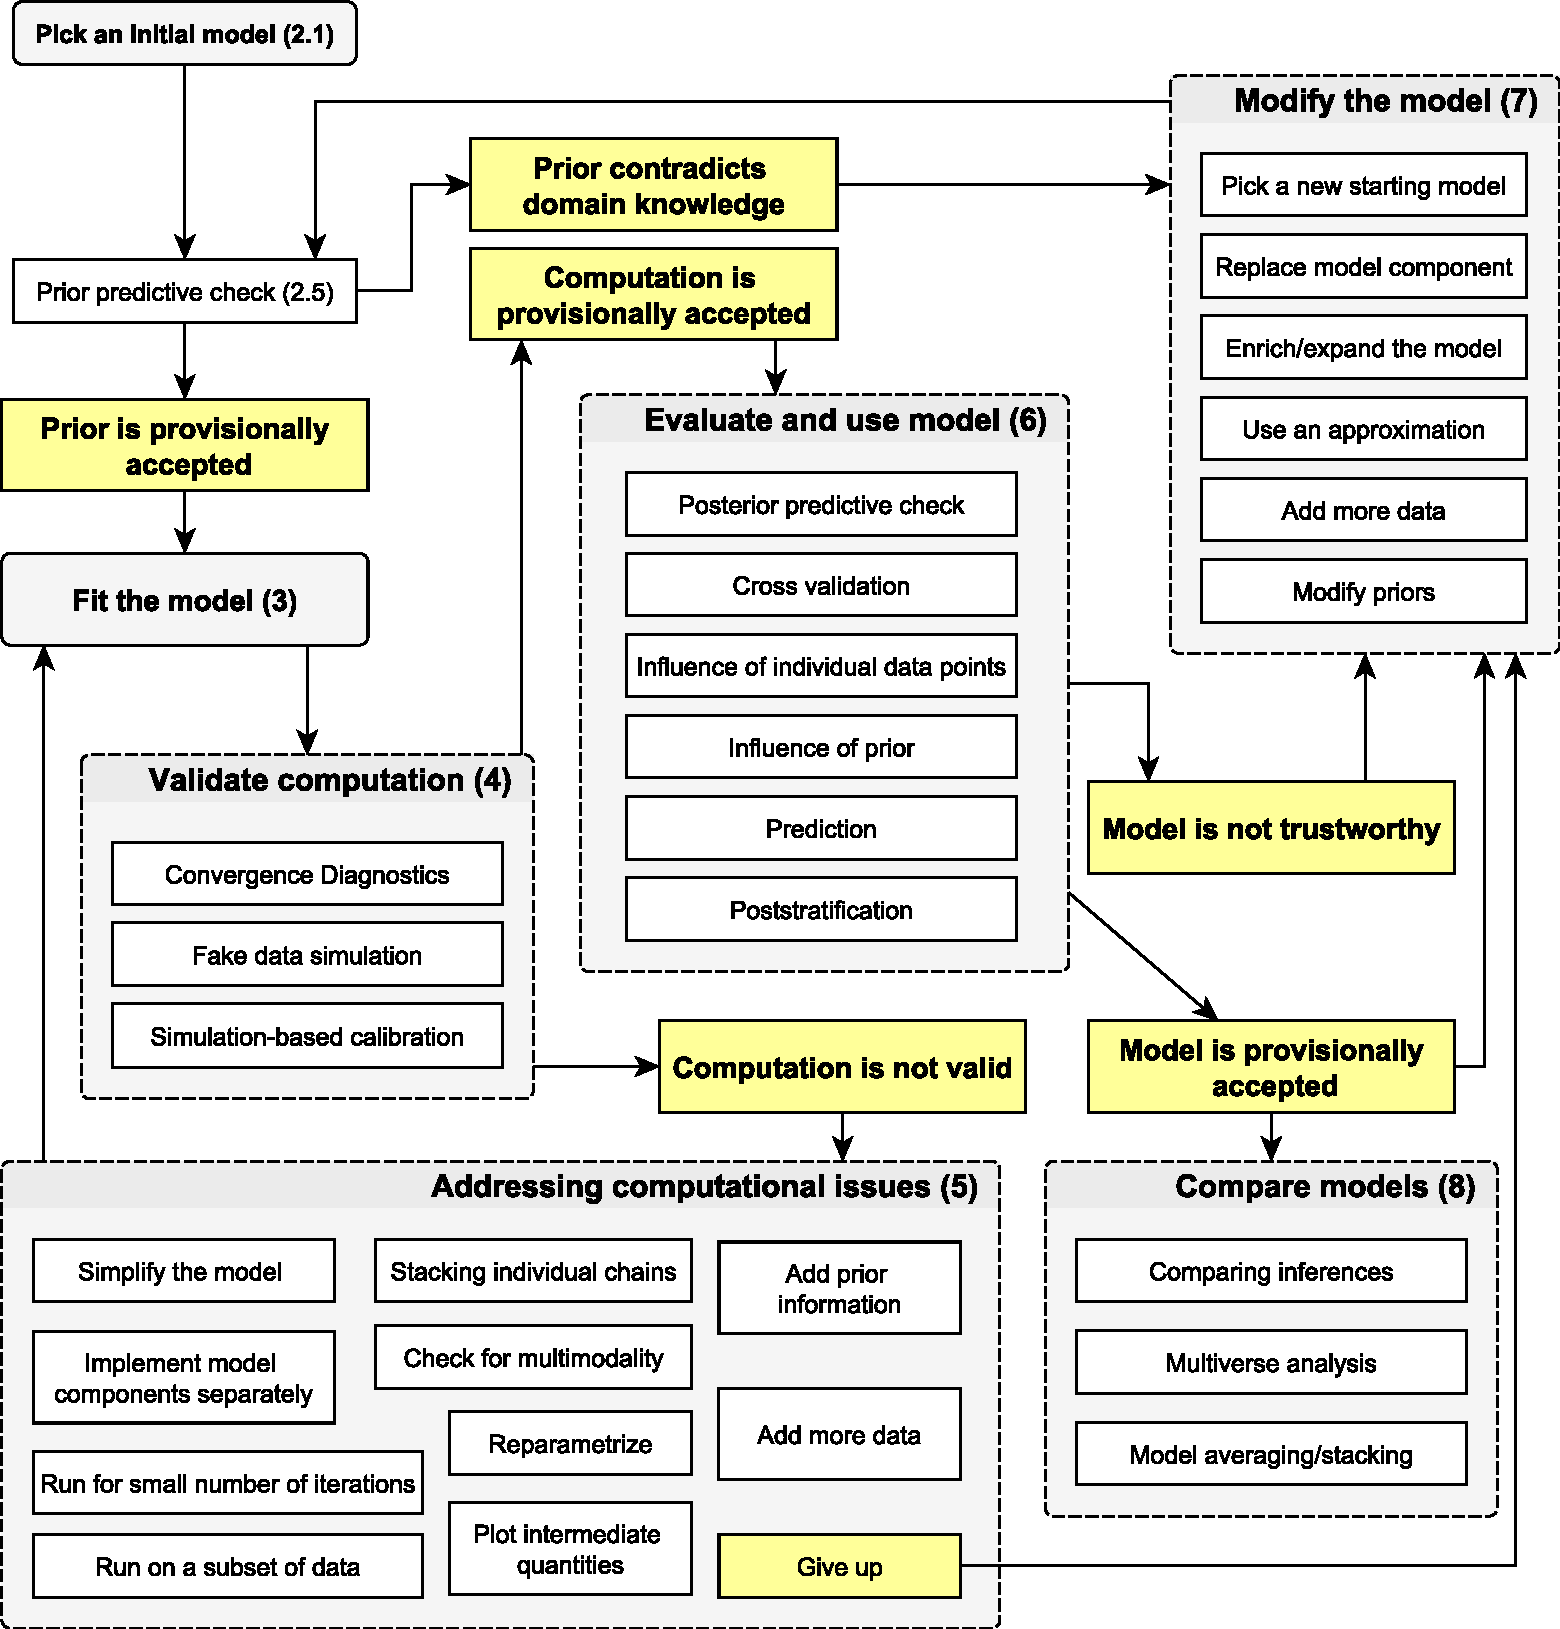
\includegraphics[width=7.5cm]{workflow_overview.pdf}
  
\end{frame}

\end{document}

%%% Local Variables: 
%%% mode: latex
%%% TeX-master: t
%%% TeX-command-extra-options: "-shell-escape"
%%% End:
